\section{Simulation Results} \label{opsimresult}

To validate that the calculations have been made correctly, an open-loop simulation of the circuit was conducted. As it can be seen in figure \ref{fig:openloop_schematic} the circuit consists of the 4 MOSFETs, the inductor, the 2 capacitors and a load. The MOSFETs are controlled with two duty cycles $D_1$ and $D_2$. FET1 and FET4 will get the actual duty cycle while FET2 and FET3 uses the complementary duty cycles. With the scope the output voltage and current through the inductor can be visualized.

\begin{figure}[H]
	\begin{center}
		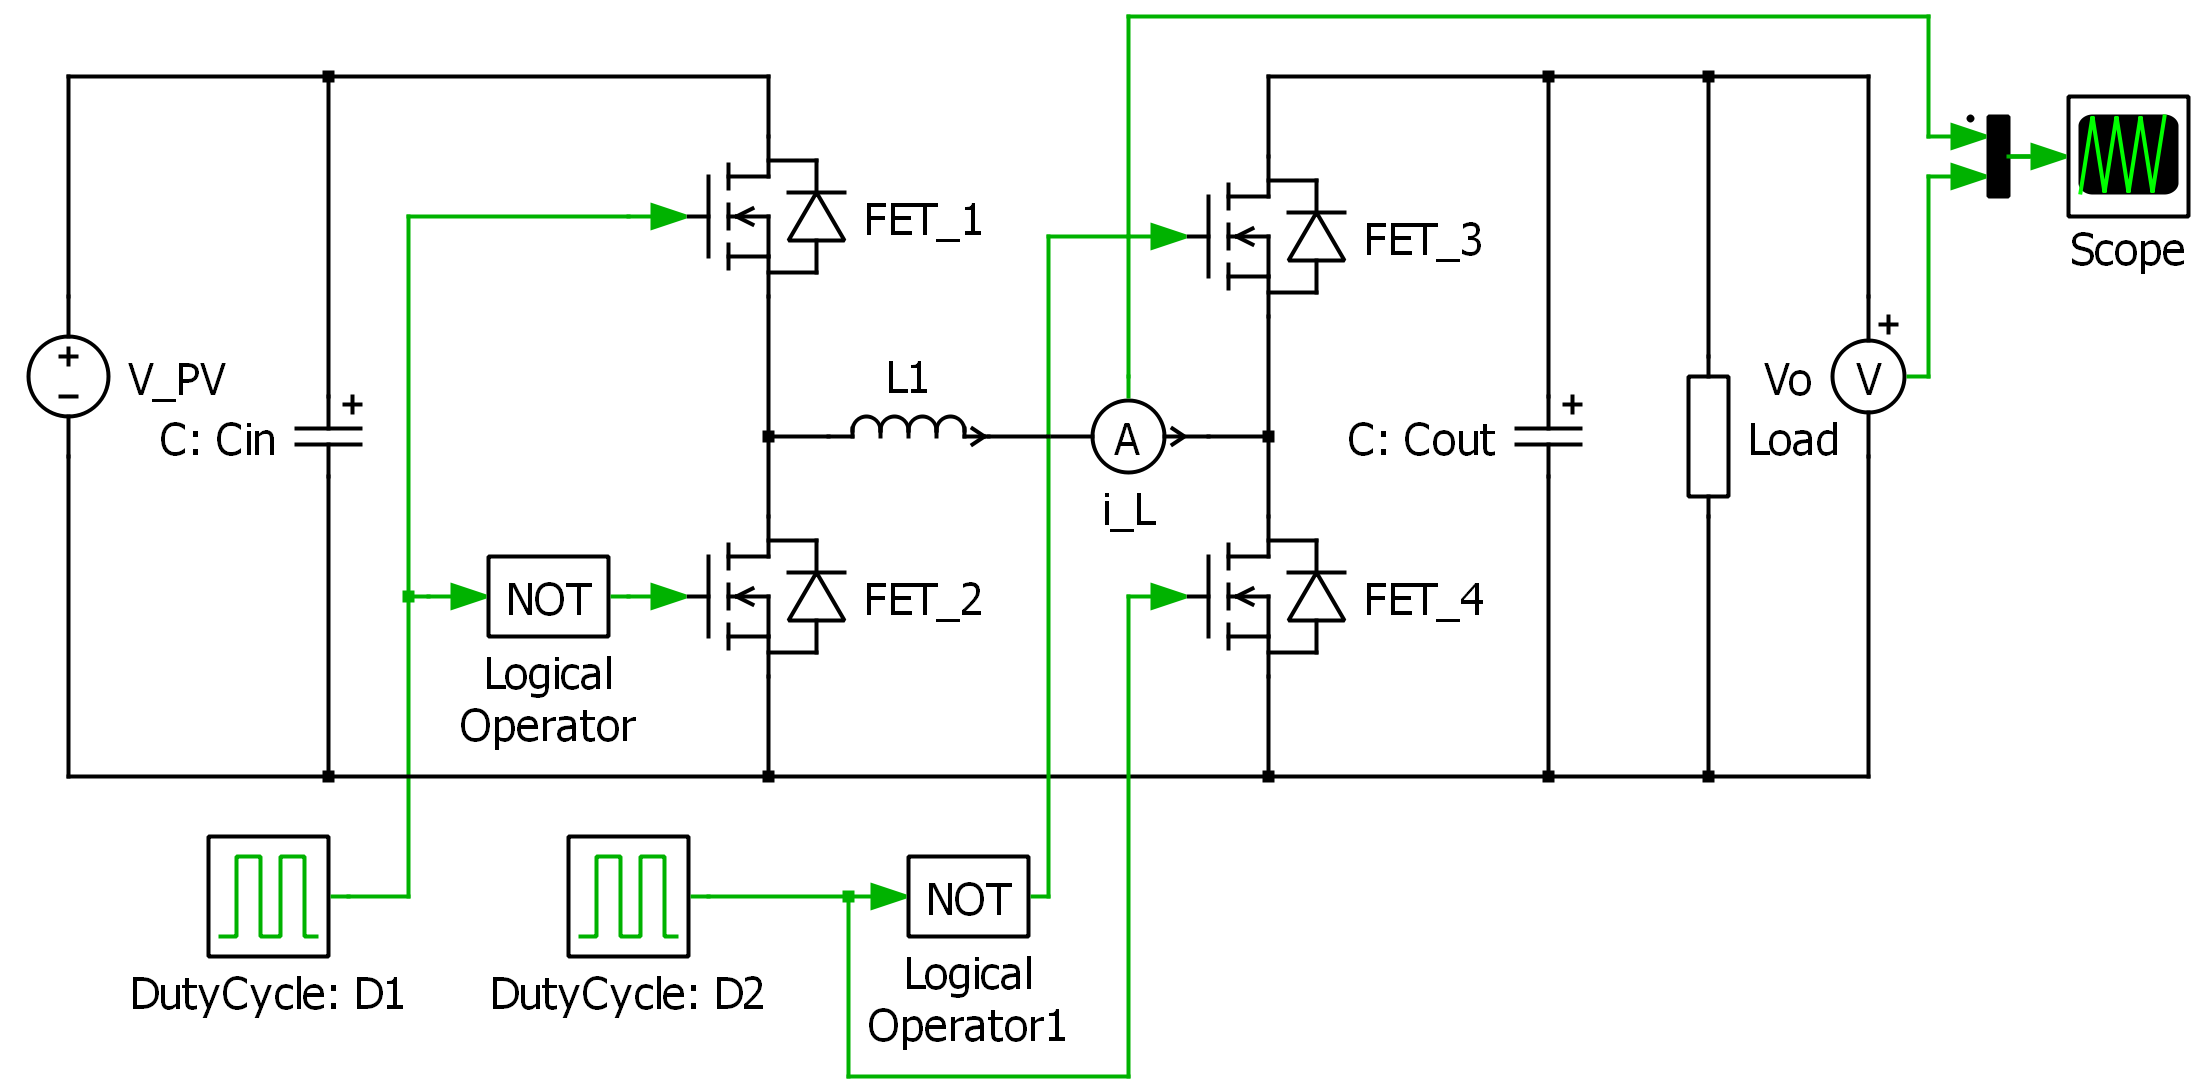
\includegraphics[width=0.7\textwidth]{../Pictures/P1/Open_loop_simulation/open_loop_schematic}
		\caption{Ideal open-loop simulation.}
		\label{fig:openloop_schematic}
	\end{center}
\end{figure}

The values for the components are $C_{in}=1.54mF$, $C_{out}=88 \mu F$ and $L_{1}=1.3mH$ as calculated in section \ref{component_sizing}. At first the buck mode is simulated. In this mode D2 is 0. This means that FET4 is off and FET3 is on. To achieve the minimum output voltage at $24V$, the corresponding duty cycle is calculated in equation \ref{eq:ol_duty_buck}. The load resistor is calculated for maximum output power for the PV panel in equation \ref{eq:ol_load_buck}.
\begin{equation} \label{eq:ol_duty_buck}
	D_1= \frac{V_{out}}{V_{in}} = \frac{24V}{36.9V} = 0.65
\end{equation}

\begin{equation} \label{eq:ol_load_buck}
	R_L = \frac{V_{out}^2}{P_{max}} = \frac{24V^2}{300W} = 1.92 \Omega
\end{equation}

%Figure \ref{fig:OL_bucksimulation} shows the output voltage and inductor current waveforms from the simulation. The initial transients are not important for an open-loop simulation and have been excluded in the figure. 
With the data obtained during simulation, the mean values are calculated such that $\widebar{V_{out}} = 23.95V$ and $\widebar{I_L} = 12.48A$. In buck mode the current through the inductor should be equal to the output current. With the values used for the simulation, the current at the output should be $12.5A$ as calculated in equation \ref{eq:Iout_buck}. The measurements show that the converter works as expected in buck mode.

\begin{equation} \label{eq:Iout_buck}
I_{out} = \frac{V_{out}}{R_{L}} = \frac{24V}{1.92\Omega} = 12.5A
\end{equation} 
  
\iffalse
\begin{figure}[H]
 	\begin{center}
 		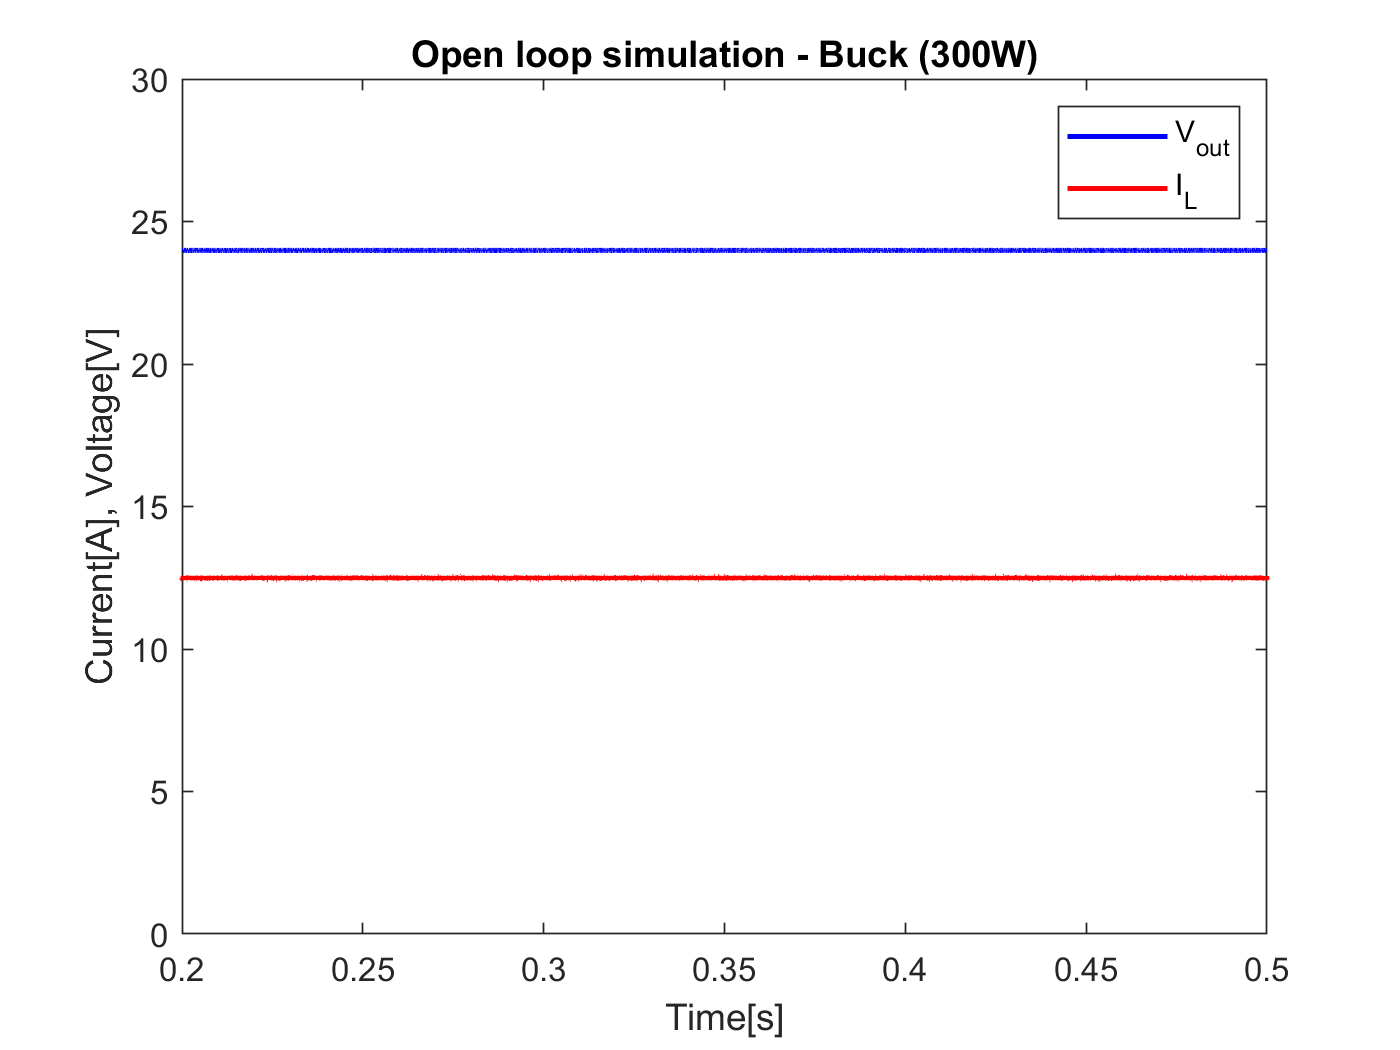
\includegraphics[width=0.6\textwidth]{../Pictures/P1/Open_loop_simulation/open_loop_buck_300W}
 		\caption{Open-loop simulation in buck mode.}
 		\label{fig:OL_bucksimulation}
 	\end{center}
\end{figure} 
\fi

The boost mode is simulated using the same values for the components and input voltage. To work in boost mode $D_1 = 1$ and $D_2$ is calculated in equation \ref{eq:boost_duty_90V} to achieve an output voltage of $90V$. The load resistor is sized in equation \ref{eq:ol_load_boost}, such that an output power of $300W$ is obtained.

\begin{equation} \label{eq:boost_duty_90V}
	D_2 = 1-\frac{V_{in}}{V_{out}} = 1 - \frac{36.9V}{90V} = 0.59
\end{equation}

\begin{equation} \label{eq:ol_load_boost}
	R_{load} = \frac{V_{out}^2}{P_{max}} = \frac{90V^2}{300W} = 27 \Omega
\end{equation}

%Figure \ref{fig:OL_boostsimulation} shows the output voltage and inductor current waveforms from the simulation. 
With the data obtained during simulation, the mean values are calculated such that $\widebar{V_{out}} = 89.95V$ and $\widebar{I_L} = 8.16A$. The theoretical current through the inductor is calculated in equation \ref{eq:IL_boost}. The measurements shows that the converter works as expected in boost mode.

\iffalse
\begin{figure}[H]
	\begin{center}
		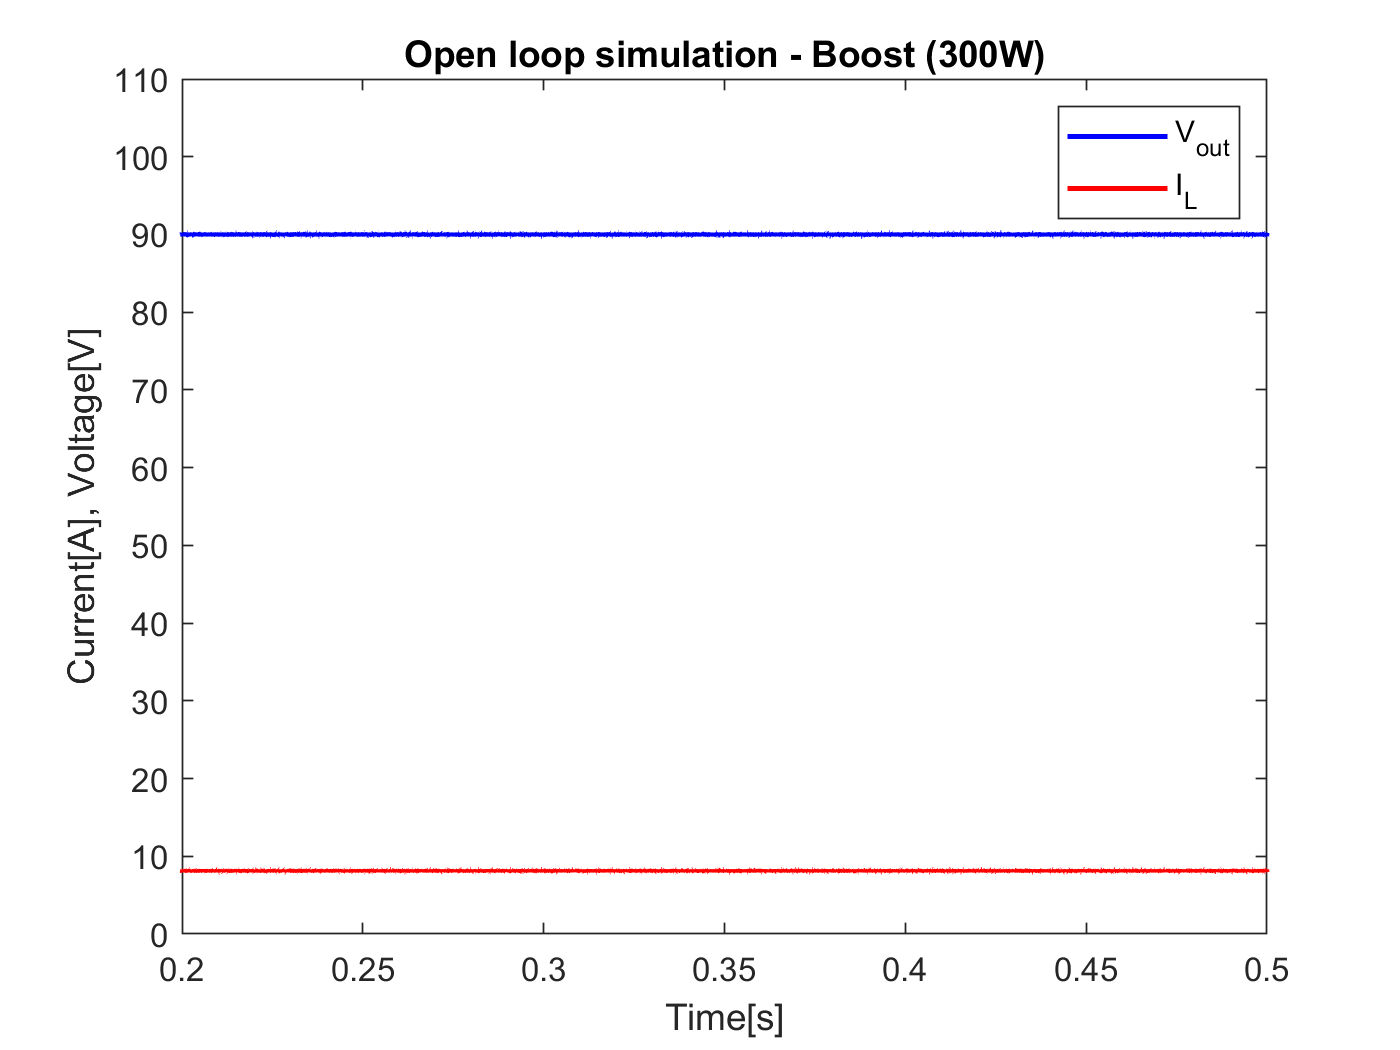
\includegraphics[width=0.6\textwidth]{../Pictures/P1/Open_loop_simulation/open_loop_boost_300W}
		\caption{Open-loop simulation in boost mode.}
		\label{fig:OL_boostsimulation}
	\end{center}
\end{figure}
\fi

\vspace{-0.6cm}
\begin{equation} \label{eq:IL_boost}
	I_L = \frac{1}{1-D} \cdot \frac{V_{out}}{R_{load}} = \frac{1}{1-0.59} \cdot \frac{90V}{27\Omega} = 8.13A
\end{equation}

The last part of the open-loop simulation is to validate the capacitor and inductor values. This is done by measuring the different ripple values under the conditions as they where calculated in section \ref{component_sizing}. The inductor is tested in boost mode with $V_{in} = 36.19V$, $D_{2} = 0.597$ and $R_{L} = 68.9\Omega$. The maximum and minimum currents are measured as $I_{max} = 3.465A$ and $I_{min} = 3.135A$, with a mean at $\widebar{I_L} = 3.3A$. The ripple current is calculated in equation \ref{eq:inductor_ripple}.

\begin{equation} \label{eq:inductor_ripple}
	\Delta I_L = \frac{I_{max}-I_{min}}{\widebar{I_L}} \cdot 100 = \frac{3.465A-3.135A}{3.3A} \cdot 100 = 10\%
\end{equation}

The output voltage ripple is also measured in boost mode, but with the maximum output power of $300W$. This means $V_{in} = 36.9V$, $D_{2} = 0.59$ and $R_{L} = 27\Omega$, as calculated during the open-loop boost simulation. The maximum and minimum voltages are measured as $V_{max} = 90.22V$ and $V_{min} = 89.77V$, with a mean at $\widebar{V_{out}} = 89.995V$. The ripple voltage is calculated in equation \ref{eq:output_voltage_ripple}.

\begin{equation} \label{eq:output_voltage_ripple}
\Delta V_{out} = \frac{V_{max}-V_{min}}{\widebar{V_{out}}} \cdot 100 = \frac{90.22V-89.77V}{89.995V} \cdot 100 = 0.5\%
\end{equation}

The input voltage ripple is measured in buck mode, with an output voltage of $24V$. This means $V_{in} = 36.9V$, $D_{1} = 0.65$ and $R_{L} = 1.92\Omega$. This simulation was done using a PV module as input source, to achieve a realistic input. The model behind the PV panel is explained in section \ref{MPPTSimulation}. The maximum and minimum voltages are measured as $V_{max} = 36.9419V$ and $V_{min} = 36.905V$, with a mean at $\widebar{V_{in}} = 36.9235V$. The ripple is calculated in equation \ref{eq:input_voltage_ripple}. The figures for the ripple measurements are included in appendix \ref{app:OL_ripple}.

\begin{equation} \label{eq:input_voltage_ripple}
\Delta V_{in} = \frac{V_{max}-V_{min}}{\widebar{V_{in}}} \cdot 100 = \frac{36.9419V-36.905V}{36.9235V} \cdot 100 = 0.099\%
\end{equation}

The analysis of the open-loop simulation results will be further explained in section \ref{ol_discussion}.